
\chapter{Chapter Zero}
We begin, not by discussing the movement of robots, but by laying out the tools needed to fully understand the problem at hand. The problem we are investigating exists in graphs, but uses topological tools to find solutions. The first two sections of the chapter serve to establish a sufficient mathematical base with which we may study the problem of autonomous movement along fixed paths.

The first section will focus on the basics of graph theory and the second will do so similarly with topology. The third extends ideas from the preceding sections in order to bridge the gap between our two primary fields of focus.

\section{Graphs}\label{sec:graphs}
%\textit{Ty's note: This section needs more comprehensive citing.}

We begin by exploring some basic elements of graph theory. A graph is a one-dimensional mathematical structure composed of edges and nodes. While graphs may be either finite or infinite, our attention will be directed at finite graphs.

\begin{defn}
A graph $G$ is the pair $G=(V,E)$ of vertices $V(G)$, usually denoted through letters or numbers, and edges $E(G)$. We say a vertex is a point in the graph and an edge is an unordered pair of vertices in $V(G)$\cite{ed}. 
\end{defn}

Graphs are useful in understanding the relationship between objects. As a result, they are used to model public transit systems, infectious diseases, communication networks, and countless other things. Since our focus is on robots which move around on a graph, let us choose to use a public transit system, specifically a railway system, as a running example.

\begin{figure}[h!]
\caption{The Graph $G$ of a Rail System}\label{fig:railgraph}
\centering
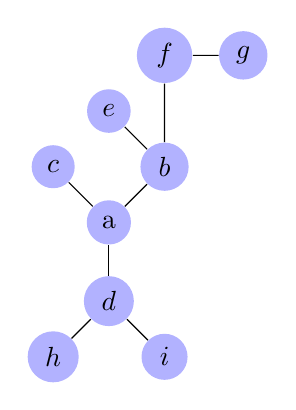
\begin{tikzpicture}
  [scale=.7,auto=left,every node/.style={circle,fill=blue!30}]
  \node (n1) {a};
  \node (n2) [above right of=n1]    {$b$};
  \node (n3) [above left of=n1]     {$c$};
  \node (n4) [below of=n1]          {$d$};
  \node (n5) [above left of=n2]     {$e$};
  \node (n6) [above right of=n5]    {$f$};
  \node (n7) [right of=n6]          {$g$};
  \node (n8) [below left of=n4]     {$h$};
  \node (n9) [below right of=n4]    {$i$};
  
    
\foreach \from/\to in
{n1/n3,n2/n1,n4/n1, n2/n5, n2/n6, n6/n7, n4/n8, n4/n9}
    \draw (\from) -> (\to);
\end{tikzpicture}
\end{figure}

Consider a train system consisting of train stations and the track which connects them. It may seem obvious then to construct a graph of some arbitrary railway system by representing nodes as stations and the tracks between them as edges. Consider the example in Figure~\ref{fig:railgraph}. Here we have a graph of a rail system with stations denoted by lettered vertices and the tracks as edges.

As we can see, our graph contains little information of physical routes traveled by trains, as each station is seemingly equidistant from one another but in actuality may be an hour or several minutes away, but the information needed as to how to effectively travel from one station to another is preserved by the relationship between edges and vertices. Even though we do not know the actual distance or time involved, it is clear from our graph that station $b$ is only one stop away from station $a$. In this case we say that $a$ and $b$ are \textbf{adjacent}.

\begin{defn}
We say that $v_x,v_y\in V(G)$ are adjacent if there exists some $e\in E(G)$ such that $e$ \textit{joins}, or connects, $v_x$ and $v_y$. Two edges are \textbf{incident} if they share a common vertex. A graph is \textbf{simple} if no two edges are incident to the same two vertices and no vertex is \textbf{adjacent} to itself.\cite{ed}
\end{defn}

\begin{figure}[h]
\centering
\caption{Not Simple and Simple Graphs}
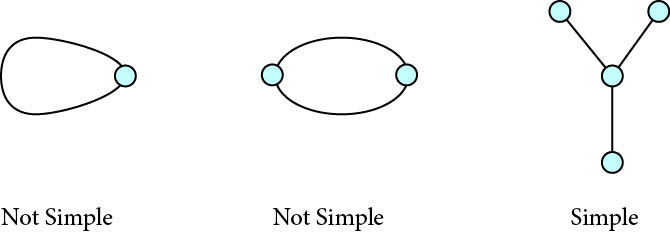
\includegraphics[scale=.5]{simples.jpg}
\label{fig:simple}
\end{figure}

In simple graphs, \textbf{degree} of a vertex $v\in V(G)$, denoted as deg$(v)$, is the number of vertices adjacent to $v$. Looking at the graph in Figure~\ref{fig:simple}, we can see that deg$(a)=3$ while deg$(f)=2$. We can classify a vertex $v$ as \textbf{essential} if deg$(v)\neq 2$. Conversely, we say vertices with degree two are \textbf{non-essential}\cite{ed}.

We define a \textbf{path} as a sequence of adjacent vertices along their incident edges such that no vertex or edge is repeated. We denote a path from $v_0$, the \textit{initial vertex}, to $v_k$, the \textit{terminal vertex}, as $(v_0,v_k)\text{-path }=v_0,e_0v_1,e_1\dots,e_{k-1},v_k$ \cite{ed}. In an abuse of notation, it is common to exclude edges from our sequence for simple graphs. A path containing $n$ vertices has length $k=n-1$.


We say a graph is \textbf{connected} if, for every $v_x,v_y \in V(G)$, there exists a path such that $v_x,v_{x+1},\dots, v_{k}=v_y$\cite{ed}. The graph in Figure \ref{fig:railgraph} is a connected graph, but it will not be if any of the edges are removed. Figure~\ref{fig:connected} shows a disconnected subgraph of the graph G from Figure~\ref{fig:railgraph}.

\begin{figure}[h]
\centering
\caption{A Disconnected Subgraph of $G$}
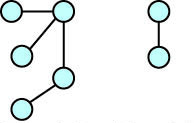
\includegraphics[scale=.5]{connected.jpg}
\label{fig:connected}
\end{figure}

For connected graphs, we can use the length of a path to define an informal metric, called the shortest path metric, defined as the path where $k$ is minimized. If we again return to Figure~\ref{fig:railgraph}, we see that the path from $g$ to $a$ is $g,f,b,a$ is shorter than the path from $d$ to $a$, which is $d, a$.

A cycle is a path such that the initial and terminal vertices are the same and no edges or vertices are repeated. Figure \ref{fig:railgraph} contains no cycles while the middle graph in Figure~\ref{fig:simple} does contain a cycle.



We can employ our understanding of a graph's paths to further classify graphs. We say a graph, such as the graph in Figure~\ref{fig:tree}, is a \textbf{tree} if it is connected and has no cycles \cite{ed}. The sub-graph of $G(V,E)$ formed by $a,b,c,$ and $d$ and their incident edges is a tree.

\begin{figure}[h]
\caption{The Tree which is a Subgraph of G}\label{fig:tree}
\centering
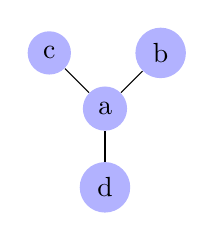
\begin{tikzpicture}
  [scale=.7,auto=left,every node/.style={circle,fill=blue!30}]
  \node (n1) {a};
  \node (n2) [above right of=n1]  {b};
  \node (n3) [above left of=n1] {c};
  \node (n4) [below of=n1] {d};

\foreach \from/\to in
{n1/n3,n2/n1,n4/n1}
    \draw (\from) -> (\to);
\end{tikzpicture}
\end{figure}


We use graphs to represent relationships between objects, but in order manipulate these relations we will need to incorporate ideas from topology.


\section{Topology}\label{sec:topology}
Topology may be broadly defined as the study of abstract mathematical space. In Section \ref{sec:graphs} we restricted ourselves to characterizing one-dimensional space, but the concepts in topology will free us from such restrictions. 

\subsection{Topological Spaces}

We begin our discussion of topology by defining a topological space.
\begin{defn}
Let $X$ be a set. We define a topology $\mathcal{T}$ on $X$ to be a collection of subsets of $X$, called open sets, such that
\begin{enumerate}
\item $X$ and $\emptyset$ are elements of $\mathcal{T}$;\
\item the union of any collection of subsets in $\T$ belongs to $\T$;\
\item the intersection of finitely many subsets in $\T$ belongs to $\T$.
\end{enumerate}
We say a set $X$, together with a topology on it, is a topological space.
\end{defn}


Formally, we define a topological space to be a space with a topology on it, $(X,\mathcal{T})$, but it is a common practice to simply say $X$ with the understanding there is a topology on it.

Let us start with a simple example, namely the finite set $X=\{1,2,3\}$. Now let us define a topology on $X$. Let $\mathcal{T}_0=\{X,\emptyset\}$. Clearly this meets the definition of a topology. We call this topology the \textit{trivial topology}. Let $X$ be the set defined above, but now let $\mathcal{T}_1=\{\emptyset, \{2\}, \{2,3\}, X\}$. This is an example of a non-trivial topology on $X$. Let us take a moment to compare the two topologies we have just constructed. Notice that $\mathcal{T}_0 \subseteq \mathcal{T}_1$. We say that $\mathcal{T}_0$ is \textbf{coarser}, or weaker, than $\mathcal{T}_1$. Similarly we say $\mathcal{T}_1$ is \textbf{finer} or stronger than $\mathcal{T}_0$. 

We can also define a topology on $\R$. Consider the collection $\mathcal{T}$ of subsets $U$ such that for every $x \in U$ there exists an $\epsilon >0$ such that $(x-\epsilon, x+\epsilon)\subset U$. We will now show this collection to be a topology.


\begin{proof}
We begin by showing that $\emptyset$ is in $\mathcal{T}$. Since there is no $x \in \emptyset$, there does not need to be an $\epsilon >0$, and so it is open. It is also clear to see that by definition $\R$ is open since for every $x$ in $\R$, there is an $\epsilon >0$ such that $(x-\epsilon, x+\epsilon) \subset \R$.

Let $U,V \subset \R$ be in $\T$ and let $W = U \cap V$. If $U$ and $V$ do not intersect, then $W=\emptyset$, which is an element of $\mathcal{T}$. Thus assume $W\neq \emptyset$. Let $x \in W$. Since $x$ is in $U$, there exists $\epsilon>0$ such that $(x-\epsilon, x+\epsilon)\subset U$ and since $x$ is in $V$ there exists $\delta>0$ such that $(x-\delta, x+\delta)\subset V$. Without loss of generality, assume that $\delta \leq \epsilon$. It follows that $(x-\delta, x+\delta) \subseteq (x-\epsilon, x+\epsilon) \subset U$. Thus $(x-\delta, x+\delta)\subset U \cap V = W$, so $U\cap V$ is an open set. For finite intersections of three or more subsets of $\R$, an inductive argument can be made.

To finish the proof we will show that the union of any collection of open sets is open. Let $A=\bigcup_{i\in I} U_i$ where ${U_i}$ is a collection of open sets in $\R$ and $i$ belongs to some index set $I$. Let $x \in A$. So there exists some $i\in I$ such that $x\in U_i$, and so there exists some $\epsilon $ such that $(x-\epsilon,x+\epsilon)\subset U_i \subseteq  \bigcup_{i\in I} U_i = A$. Thus the union of any collection of subsets in $\mathcal{T}$ belongs to $\mathcal{T}$.

Since the collection of open sets $\T$ satisfies all three conditions of a topology, $\T$ is a topology on $\R$. 
\end{proof}

We say this particular $\T$ is the standard topology on $\R$. 

The previous proof demonstrated the construction of the standard topology on the real line, but what we did not mention is that the open sets $U$ are \textbf{neighborhoods} of points in them.  

\begin{defn}
Let $X$ be a topological space and $x\in X$. An open set $U$ containing $x$ is said to be a neighborhood of $x$.
\end{defn}


This is a powerful definition, principally because it helps us determine if a set is open or not, which will aid us as we explore topology in greater depth.

In the proof above we showed the entire collection of open sets satisfied the definition for a topology. This may seem intuitive for familiar spaces such as $\R$, but for less familiar or more complicated spaces it may be more challenging. Instead, we can define a smaller collection of open sets called a \textbf{basis} and then use it to generate the remaining open sets in the topology.

\begin{defn}
Let $X$ be a set and let $\mathbb{B}$ be a collection of subsets of $X$. The collection $\mathbb{B}$ is a basis for a topology on $X$ if the following conditions are satisfied:
\begin{enumerate}
\item for $x\in X$ there exists some $B\in \mathbb{B}$ such that $x\in B$.
\item if \textbf{basis elements} $B_1, B_2 \in \mathbb{B}$ and $x\in B_1 \cap B_2$, there exists some $B_3$ such that $x \in B_3 \subseteq B_1 \cap B_2$.\cite{top}
\end{enumerate}
\end{defn}

Simply put, every element in $X$ is in a basis element and every element in the intersection of two basis elements is contained in a basis element which is a subset of the intersection.

Having examined the definition of a basis, we are now free to use it in defining a topology on a set.

\begin{defn}
Let $\B$ be a basis on $X$. The \textbf{topology $\T$ generated by $\B$} is obtained by defining the open sets to be the empty set and every set equal to the union of basis elements.
\end{defn}

Having multiple techniques to define topologies has two immediate benefits. The first is that defining a topology in terms of the basis which generates it is in many cases more tractable than showing the entire collection of open sets to be a topology. For the general proof of this we refer the reader to page $48$ of \cite{top}.

While we refer the reader for general proof, we can demonstrate it by generating the standard topology on the real line. Let $$\mathbb{B}=\{ (a,b)\subseteq \R| a<b\},$$ which is the set of all open intervals. Clearly each $x\in \R$ is contained in some $B\in \mathbb{B}$, so our first condition is satisfied. Now consider the basis elements $B_1, B_2\in \mathbb{B}$. If their intersection is not the empty set, $B_1\cap B_2 \neq \emptyset$, then there will always exist an interval, $B_3$, around every point in the intersection. Thus we have shown that $\mathbb{B}$ is a basis for a topology on $\R$. 


It can be further shown that a set which is the union of basis elements is open in the standard topology on $\R$ and conversely every open set in the standard topology can be written as a union of these basis elements. Hence the topology generated by this basis is the standard topology on $\R$.

We can also use bases to generate a topology on the product of two spaces. Given two  topological spaces, $X$ and $Y$, we say the product topology on $X\times Y$ is generated by the basis
$$\mathbb{B}=\{U\times V|\text{ } U \text{ is open in } X \text{ and } V \text{ is open in }Y\}.$$

In a similar manner as to how we generate topologies from a basis, we can generate product topologies from the product of bases. Explicitly, we claim that if $\mathbb{C}$ is a basis for $X$ and $\mathbb{D}$ is a basis for $Y$, then $$\mathbb{E}=\{ C\times D |\text{ }C\in \mathbb{C} \text{ and } D\in \mathbb{D}\}$$ is a basis for $X\times Y$. For the proof of this, please consult page 101 in \cite{top}.

\subsection{Homeomorphism and Homotopy Equivalence }
Having established a rudimentary basis of topology, we now possess the tools to extend ideas from other fields of mathematics into our current area of interest. In an introductory analysis course, one of the first things students learn is how to determine if a function is continuous or not. We call this definition of a continuous function the \textbf{epsilon-delta definition of continuity}. 

While this definition holds up well for spaces such as the real line, we need to be able to generally define continuity on any topological space. As a result, we have an equivalent definition of continuity called the \textbf{open set definition of continuity}\cite{top}.

\begin{defn}
Let $X$ and $Y$ be topological spaces. A function $f\colon X \rightarrow Y$ is continuous if and only if for every open set $V$ in $Y$, $f^{-1}(V)$ is open in $X$ . 
\end{defn}

Let us acclimate to this definition of continuity by showing the identity function $I_X\colon X\rightarrow X$ to be continuous on any topological space $X$. Let $U$ be open in the topology on $X$. Define $I_X$ to be the identity function given by $I_X(x)=x$ for all $x\in X$. Since for all $x\in U$ we have $I^{-1}_X(x)=x$, $I^{-1}_X(U)=U$ is open in $X$. Thus $I_X$ is continuous. 

We can also show that the composition of continuous functions is continuous. 

\begin{prop}\label{prop:cont}
The composition of continuous functions is continuous. 
\end{prop}

\begin{proof}
Let $X,Y,$ and $Z$ be topological spaces. Let $f\colon X \rightarrow Y$ and $g\colon Y\rightarrow Z$ be continuous. Let $U \subseteq Z$ be an open set. In order to prove that $g\circ f$ is continuous, we need to show that $(g\circ f)^{-1}(U)$ is open in $X$. Since we know that $g$ is continuous, we know $g^-1(U)$ to be open in $Y$. Similarly, since $f$ continuous, we know that $f^{-1}(g^{-1}(U))$ is open in $X$. So $f^{-1}(g^{-1}(U))=(g\circ f)^{-1}(U)$, we have shown $(g\circ f)^{-1}(U)$ to be open in $X$. Thus the composition of continuous functions is continuous. 
\end{proof}

Often in mathematics, we are interested in classifying and comparing mathematical objects. In topology, we use continuity to classify and compare topological spaces. By constructing a continuous function between two spaces, we are able to move beyond their superficial differences and compare their underlying \textit{structure} or topological properties. We call continuous bijections between topological spaces \textbf{homeomorphisms} if their inverse is also continuous.


\begin{defn}
Let $X$ and $Y$ be topological spaces, and let $f\colon X\rightarrow Y$ be a bijection with inverse $f^{-1}\colon Y \rightarrow X$. If both $f$ and $f^{-1}$ are continuous then we call $f$ a homeomorphism and say there is a homeomorphism between $X$ and $Y$. We also say that $X$ and $Y$ are homoemorphic or topologically equivalent. We denote this as $X\cong Y$. 
\end{defn}

\begin{prop}
The relation ``homeomorphism" is an equivalence relation on the set of all topological spaces.
\end{prop}

\begin{proof}
Recall that a relation on any given set is considered an equivalence relation if and only if it is reflexive, transitive, and symmetric. Let $X$, $Y$, and $Z$ be topological spaces.

We will begin by verifying reflexivity. Since we have previously shown the identity function to be continuous and since it is a bijection and the inverse of $I_X$ is itself by definition, $I_X$ is a homeomorphism and $X\cong X$. 

Next we will demonstrate transitivity. Let  $f\colon X\rightarrow Y $ and $g\colon Y\rightarrow Z$ be homeomorphisms. We define $h\colon X\rightarrow Z$ by $h=g\circ f$. We know the composition of two continuous bijections to be a continuous bijection. We also know that $h^{-1}=f^{-1}\circ g^{-1}$ is continuous because $f^{-1}$ and $g^{-1}$ are continuous. Hence $h$ is a homeomorphism.

The last step is to show symmetry. Let $X\cong Y$. By definition there exists a homeomorphism $f\colon X \rightarrow Y$. By the definition of homeomorphism, we know that $f^{-1}$ is a continuous bijection and its inverse $f$ is continuous, and so $f^{-1}$ is a homeomorphism from $Y$ to $X$. Thus we have shown if $X\cong Y$ then $Y\cong X$.

Since the homeomorphism relation is reflexive, transitive, and symmetric, it is an equivalence relation.
\end{proof}

We can conceptualize homeomorphisms as the bending or stretching of one space into another without intersecting or tearing the space. Consider the real line $\R$ and the interval $(-1,1)$. We can compress the real line down until it is the interval $(-1,1)$. The explicit function for doing so is given by $f(x)=\frac{x}{|x|+1}$, which can be shown to be a continuous bijection with a continuous inverse. Thus $\R$ is homeomorphic to $(-1,1)$. For the complete proof, please consult page $143$ of \cite{top}. 

To compare the topological structure of spaces, we attempt to construct homeomorphisms between them. However, we can also compare continuous functions between two topological spaces. This defines an equivalence class on the set of all continuous functions from $X$ to $Y$ known as \textbf{homotopy equivalence}.


\begin{defn}
Let $X$ and $Y$ be topological spaces, $f,g\colon X \rightarrow Y$ be continuous functions, and $I=[0,1]$. We say that $f$ and $g$ are homotopic, or that a homotopy exists between them, if we can construct a continuous function $F\colon X \times I \rightarrow Y$ such that $F(x,0)=f(x)$ and $F(x,1)=g(x)$ for each $x \in X$. We denote a homotopy as $f \simeq g$.
\end{defn}

\begin{prop}
The relation ``homotopy" is an equivalence relation on the set of all continuous functions from $X$ to $Y$.
\end{prop}

\begin{proof}
We show the homotopic relation to be an equivalence relation on the set of all continuous functions from $X$ to $Y$. Let $X$ and $Y$ be topological spaces and let $f,g\colon X \rightarrow Y$ be continuous functions. 

We begin by showing that $f\simeq f$. Let $F\colon X \times I \rightarrow X$ be defined by $F(x,t)=f(x)$. We know that $f$ is continuous, and we know that for all $t$, $F(x,t)=f(x)$. Thus $F$ is continuous and $f\simeq f$.

We will now show if $f\simeq g$ and $g \simeq h$, then $f \simeq h$. Assume a homotopy exists between $f$ and $g$, defined as $F\colon X\times I \rightarrow Y$, and $g$ and $h$, defined as $G\colon Y\times I \rightarrow Y$. We construct $H\colon X\times I \rightarrow Z$ defined as 
\begin{displaymath}
   H(x,t) = \left\{
     \begin{array}{lr}
       F(x,2t)  &   \text{if } 0\leq t\leq \frac{1}{2},\\
       G(x,2t-1) &  \text{ if } \frac{1}{2}\leq t\leq 1\text{.}
     \end{array}
   \right.
\end{displaymath} 

Since $F$ and $G$ are continuous functions, then by the Pasting Lemma we know $H$ is a continuous function. For the proof of the Pasting Lemma, see page 137 in \cite{top}. Thus we have shown that given $f\simeq g$ and $g \simeq h$, $f \simeq h$.

To finish, we will demonstrate symmetry. Assume $f\simeq g$, thus $F\colon X \times I \rightarrow Y$ is a homotopy. Define $H\colon X \times I \rightarrow X \times I$ given as $H(x,t) = (x, 1-t)$. Using the product topology on $X\times I$, it can be shown that $H$ is continuous. Define $G\colon X\times I \rightarrow Y$ as $G= F\circ H$, which is explicitly given as $G(x,t)=F(x,1-t)$. Since $G$ is the composition of continuous functions, we know it to be continuous by Proposition~\ref{prop:cont}. Since $G(x,0)=g(x)$ and $G(x,1)=f(x)$, $G$ is a homotopy and so we have shown the homotopy relation to be symmetric.

Since a homotopy satisfies the three conditions of an equivalence relation, $f\simeq g$ is an equivalence relation.
\end{proof}

Taking the product of the domain and the unit interval may seem odd at first, but it actually can aid our intuition. We may think of a homotopy as a movie, with the unit interval behaving like time as the reel runs down. At the start of our film, our function is $f$, but as time goes on it is gradually deformed into $g$. 

We should note that we may only define a homotopy between functions that have the same domain and co-domains. However, we say two spaces, $X$ and $Y$, are homotopy equivalent, or homotopic, if and only if they are both deformation retracts of finer space $Z$. In this way, we can think about homotopy equivalence as a finer classification of spaces than homeomorphisms. 

We will show this by explicitly constructing an homotopy between the open ball, $B^1 =\{x \in \R| \text{ }|x| <1\}$, and the point $\{0\}\subset \R$. Let $f\colon B^1 \rightarrow \R$ be defined as $f(x)=x$ and let $g\colon B^1 \rightarrow \R$ be given as $g(x)=0$. We know that $f$ is a continuous function since we have shown $I_X$ to be continuous. We also know that $g$ is continuous since it is a constant function. We now define our homotopy $F\colon B^1 \times I \rightarrow \R$ to be $F(x,t)= (1-t)x$. It can be shown that the product of two continuous functions is also continuous. For the outline of this proof, please consult page 139 of \cite{top}. Since we know the product of continuous functions to be continuous, $F$ is thus continuous. 

Since we have shown $F$ to be continuous, we verify that $F(x,0)= (1-0)f(x) = f(x)$ and $F(x,1)= 0 =g(x)$, and thus $F$ is a homotopy and $f\simeq g$.  

Hopefully the previous example demonstrates the differences between a homeomorphism and a homotopy. We may picture $F$ to gradually retract $B^1$ into the the point $\{0\}$. We call this gradual shrinking of a set onto its subset a \textbf{deformation retract}.

\begin{defn}
Let $X$ be a topological space with $A\subseteq X$, let $i\colon A\hookrightarrow X$ be the inclusion function, the function given by $i(a)=a$ for every $a$ in $A$, and let $f\colon X\rightarrow A$ be a continuous function such that $f(a)= a$ for all $a\in A$. We say $A$ is a deformation retract of $X$ and that function $i\circ f\colon X\rightarrow X$ is a deformation retraction if $i\circ f \simeq I_X$ such that the homotopy function fixes every point in $A$.
\end{defn}

Let us take a moment to fully explore this definition. For $i \circ f$ to be a deformation retraction, there must exist a homotopy $F\colon X\times I \rightarrow X$ which satisfies the following conditions:
\begin{enumerate}
\item $F(x,0)=I_X(x)=x$ for all $x \in X$;

\item $F(x,1)=f(x)=i(f(x))$ for all $x\in X$;

\item $F$ is continuous;
\item $F(a,t)=a$ for all $t$ and for all $a$ in $A$.
\end{enumerate}

This section was constructed in order to define homotopy and deformation retracts. These are powerful tools which allow us to distort and simplify topological spaces, however, just as we developed the notion of a basis so that we could generate a topology from it, we will see in the next section that we can also construct spaces around homotopy types and deformation retracts.



\section{CW Complexes}
The problem of collision avoidance along fixed movement networks exists in graph theory, but we rely on topological tools to determine solutions. To create the crucial link between these two fields, we will employ CW complexes. As with graphs, CW complexes may be either finite or infinite, but for the purposes of this thesis we will only focus our attention on the finite case.

%fixed path movement
\begin{defn}
The closed $n$-ball is defined as $$D^n=\{\textbf{x}=(x_1,x_2,\dots, x_n)\in \R^n |\text{  } |\textbf{x}| \leq 1 \text{ where} |x|=\sqrt x_1^2+\cdots x_n^2
 \};$$ the boundary of the closed \n-ball is defined as the $(n-1)$-sphere given by $$ S^{n-1} = \{\textbf{x}\in D^n | \text{  } |\textbf{x}|=1\};$$ and their difference is the open \n-ball, denoted $B^n$, defined as $$B^n = D^n \setminus S^{n-1} = \{\textbf{x}\in D^n | \text{  } |\textbf{x}|< 1\}.$$ 
\end{defn}
Note that we can rearrange the definition of an open \n-ball to define a closed \n-ball as $D^n= B^n \cup S^{n-1}$. 

While the term boundary has a more general definition, we will only be using it within the context of CW complexes and so define it only in context. For the explicit definition, please consult \cite{top}.


Having established a rigorous definition for \n-balls, we generalize our understanding to obtain a definition of an \textbf{\n-cell}.

\begin{defn}
A subspace $e$ of of a topological space $X$ is considered an $n$-dimensional cell, called an \n-cell, in $X$ if it is homeomorphic to the open $n$-ball, $B^n$. We also define $e$ to be a \textbf{closed \n-cell} in $X$ if it is the union of an open \n-cell and its boundary, $(n-1)$-cell homeomorphic to $S^{n-1}$. In other words, $e$ is a closed $n$-cell if it is homeomorphic to $D^n$. Unless otherwise stated so, an $n$-cell is an open $n$-cell. 
\end{defn}

While we still lack the tools to formally define a CW complex, we are moving in the right direction. We can intuit CW complexes as the union of disjoint open cells \cite{cw}.

Let us explore our newfound intuition by demonstrating that a closed $1$-cell is the disjoint union of $B^1 \cup S^0$. Let us state the sets explicitly;
\begin{align*}
D^1 &= B^1 \cup S^0\\
D^1 &= (-1,1) \cup \{-1,1\}.
\end{align*}

Next, we partition $\{-1,1\}$ into $\{-1\}\cup\{1\}$. Thus we have $$D^1 = (-1,1) \cup \{-1\}\cup\{1\},$$ which is a union of distinct open cells. Referring back to the previous definition, it is clear that $B^1$ is an open $1$-cell and $D^1$ is the closed $1$-cell.

Having accustomed ourselves to working with a closed $1$-cell, we can now generalize our previous method for any closed $n$-cells where $n\geq 1$.

Let us now take a moment to examine Figure~5 to help us in digesting the preceding formalism.

\begin{figure}[h]
\label{fig:nwacells}
\centering
\caption{A $0$-cell, a Closed $1$-Cell, and a Closed $2$-Cell}
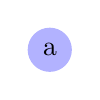
\begin{tikzpicture}
  [scale=.8,auto=left,every node/.style={circle,fill=blue!30}]
  \node (n1) {a};

\end{tikzpicture}
\hspace{.5in}
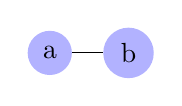
\begin{tikzpicture}
  [scale=.8,auto=left,every node/.style={circle,fill=blue!30}]
  \node (n1) {a};
  \node (n2) [right of=n1]  {b};

\foreach \from/\to in
{n1/n2}
    \draw (\from) -> (\to);
\end{tikzpicture}
\hspace{.5in}
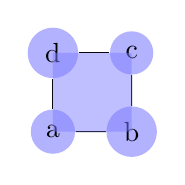
\begin{tikzpicture}
  [scale=.8,auto=left,every node/.style={circle,fill=blue!30}]
  \node (n1)                {d};
  \node (n2) [right of=n1]  {c};
  \node (n3) [below of=n2]  {b};
  \node (n4) [below of=n1]  {a};

\foreach \from/\to in
{n1/n2, n2/n3, n3/n4, n4/n1}
    \draw (\from) -> (\to);
    \path[fill=blue!50,opacity=.5] (n1.center) to (n2.center) to (n3.center) to (n4.center) to (n1.center);
\end{tikzpicture}
\end{figure}
%\printbibliography

The leftmost object is a $0$-cell. As we have discussed before, we may think of a $0$-cell as a point. The middle object is a closed $1$-cell. It is plain to see that the open $1$-cell is the line between $0$-cells labeled $a$ and $b$, which is the open $1$-cell's boundary. The rightmost object is a closed $2$-cell. The shaded region is the open $2$-cell which is enclosed by four closed $1$-cells which are neatly glued together.

There is, however, something more going on here. Let us consider all three objects at once; specifically we should pay close attention to the progression from left to right. Notice how the $1$-cell is built from the $0$-cell and how the $2$-cell is extended from the $1$-cell. We can iterate this process forward one step to describe a $3$-cell. The closed $3$-cell, the cube, is formed from the union of the open $3$-cell with a boundary cube consisting of six nicely attached closed $2$-cells. 

Expanding on the previous observation, we may now construct a space $X$ composed of $n$-cells. Our construction has three distinct steps;
\begin{enumerate}
\item We begin by considering the collection of $0$-cells and call it $X^0$. Referring back to Figure 5, $X^0$ for the $2$-cell would simply $X^0=\{a,b,c,d\}$. At this stage, we can think about the $2$-cell as simply the four vertices.

\item We then inductively form $X^n$ from the \textbf{$n$-skeleton}, the collection of $m$-cells where $m<n$, by building off of $X^{n-1}$. We do this by attaching open $n$-cells $e^n_\alpha$ via distinct maps $f_\alpha \colon S^{n-1} \rightarrow X^{n-1}$, where $\alpha$ is an index on the set of all $n$-cells. This process generates the closed $n$-cells of $X^n$ by attaching the boundary of each $n$-cell to its the corresponding cells of the $n$-skeleton.

We can visualize this step for the $2$-cell as follows. We begin by attaching a $1$-cell to every pair of vertices. This ``fills in" the edges of our square. We then map $B^2$ to the interior of the square whose boundary is formed by the connected $1$-cells. Our two-cell is now complete.

If we think about it like a movie, we start with our $0$-cells, which are then connected by $1$-cells which extend from a vertex over to join another, thus forming edges. Then our square is gradually filled in.

%Equivalently, $X^n = X^{n-1} \bigcup_\alpha e^n_\alpha$ where every $e^n_\alpha$ is an open n-ball.


\item Since we are only interested in finite spaces, we let $X=X^n$ for some $n<\infty$. This results in the eventual termination of the inductive construction.
\end{enumerate}

Spaces constructed in this fashion are called $\textbf{CW complexes}$\cite{at}. \\

The value in defining graphs in terms of CW complexes will soon become abundantly clear, but we can glean important implications from our definition. 

The primary result is that CW complexes are easily expandable because they are built from the permutations of lower dimensional CW complexes without altering their fundamental structure \cite{cw}. Let us briefly return to our discussion on graph theory. Recall the definition of a tree. If we were to use trees in order to model robotic movement and suddenly needed to expand our movement space, then we would need to be very careful in how we added vertices and edges for fear of our graph no longer satisfying the definition of a tree. No such care is needed with CW complexes.

The formal definition of a CW complex relies on topological tools outside the scope of this work. For curious readers wishing to learn more, we refer you to either \cite{at} or \cite{cw}.

The tree seen in Section~\ref{sec:graphs} is $\Y$, which can be thought of as a one-dimensional CW complex consisting of three $1$-cells which are attached at their common boundary. We begin with the vertices of $\Y$. These vertices make up $X^0$. We then attach the $1$-cells to their boundaries, thus giving us the edges.

\begin{figure}[h]
\centering
\caption{The Graph $\Y$ as a CW Complex}
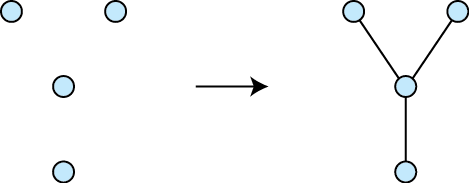
\includegraphics[scale=.75]{CW_Y}
\label{fig:cw_y}
\end{figure}

Since this CW complex is composed of only $1$- and $0$-cells, it will be one-dimensional. If we wished to expand this CW complex, we can take the product of $\Y$ with itself in order to form the product CW complex, which we will illustrate in the following chapter.

While the actual definition of a CW complex still evades us, our interest lies in their application and so we will exchange rigor for convenience as we begin to apply our newfound mathematical tools to building a movement space for robots.